\documentclass[1p]{elsarticle_modified}
%\bibliographystyle{elsarticle-num}

%\usepackage[colorlinks]{hyperref}
%\usepackage{abbrmath_seonhwa} %\Abb, \Ascr, \Acal ,\Abf, \Afrak
\usepackage{amsfonts}
\usepackage{amssymb}
\usepackage{amsmath}
\usepackage{amsthm}
\usepackage{scalefnt}
\usepackage{amsbsy}
\usepackage{kotex}
\usepackage{caption}
\usepackage{subfig}
\usepackage{color}
\usepackage{graphicx}
\usepackage{xcolor} %% white, black, red, green, blue, cyan, magenta, yellow
\usepackage{float}
\usepackage{setspace}
\usepackage{hyperref}

\usepackage{tikz}
\usetikzlibrary{arrows}

\usepackage{multirow}
\usepackage{array} % fixed length table
\usepackage{hhline}

%%%%%%%%%%%%%%%%%%%%%
\makeatletter
\renewcommand*\env@matrix[1][\arraystretch]{%
	\edef\arraystretch{#1}%
	\hskip -\arraycolsep
	\let\@ifnextchar\new@ifnextchar
	\array{*\c@MaxMatrixCols c}}
\makeatother %https://tex.stackexchange.com/questions/14071/how-can-i-increase-the-line-spacing-in-a-matrix
%%%%%%%%%%%%%%%

\usepackage[normalem]{ulem}

\newcommand{\msout}[1]{\ifmmode\text{\sout{\ensuremath{#1}}}\else\sout{#1}\fi}
%SOURCE: \msout is \stkout macro in https://tex.stackexchange.com/questions/20609/strikeout-in-math-mode

\newcommand{\cancel}[1]{
	\ifmmode
	{\color{red}\msout{#1}}
	\else
	{\color{red}\sout{#1}}
	\fi
}

\newcommand{\add}[1]{
	{\color{blue}\uwave{#1}}
}

\newcommand{\replace}[2]{
	\ifmmode
	{\color{red}\msout{#1}}{\color{blue}\uwave{#2}}
	\else
	{\color{red}\sout{#1}}{\color{blue}\uwave{#2}}
	\fi
}

\newcommand{\Sol}{\mathcal{S}} %segment
\newcommand{\D}{D} %diagram
\newcommand{\A}{\mathcal{A}} %arc


%%%%%%%%%%%%%%%%%%%%%%%%%%%%%5 test

\def\sl{\operatorname{\textup{SL}}(2,\Cbb)}
\def\psl{\operatorname{\textup{PSL}}(2,\Cbb)}
\def\quan{\mkern 1mu \triangleright \mkern 1mu}

\theoremstyle{definition}
\newtheorem{thm}{Theorem}[section]
\newtheorem{prop}[thm]{Proposition}
\newtheorem{lem}[thm]{Lemma}
\newtheorem{ques}[thm]{Question}
\newtheorem{cor}[thm]{Corollary}
\newtheorem{defn}[thm]{Definition}
\newtheorem{exam}[thm]{Example}
\newtheorem{rmk}[thm]{Remark}
\newtheorem{alg}[thm]{Algorithm}

\newcommand{\I}{\sqrt{-1}}
\begin{document}

%\begin{frontmatter}
%
%\title{Boundary parabolic representations of knots up to 8 crossings}
%
%%% Group authors per affiliation:
%\author{Yunhi Cho} 
%\address{Department of Mathematics, University of Seoul, Seoul, Korea}
%\ead{yhcho@uos.ac.kr}
%
%
%\author{Seonhwa Kim} %\fnref{s_kim}}
%\address{Center for Geometry and Physics, Institute for Basic Science, Pohang, 37673, Korea}
%\ead{ryeona17@ibs.re.kr}
%
%\author{Hyuk Kim}
%\address{Department of Mathematical Sciences, Seoul National University, Seoul 08826, Korea}
%\ead{hyukkim@snu.ac.kr}
%
%\author{Seokbeom Yoon}
%\address{Department of Mathematical Sciences, Seoul National University, Seoul, 08826,  Korea}
%\ead{sbyoon15@snu.ac.kr}
%
%\begin{abstract}
%We find all boundary parabolic representation of knots up to 8 crossings.
%
%\end{abstract}
%\begin{keyword}
%    \MSC[2010] 57M25 
%\end{keyword}
%
%\end{frontmatter}

%\linenumbers
%\tableofcontents
%
\newcommand\colored[1]{\textcolor{white}{\rule[-0.35ex]{0.8em}{1.4ex}}\kern-0.8em\color{red} #1}%
%\newcommand\colored[1]{\textcolor{white}{ #1}\kern-2.17ex	\textcolor{white}{ #1}\kern-1.81ex	\textcolor{white}{ #1}\kern-2.15ex\color{red}#1	}

{\Large $\underline{12a_{1002}~(K12a_{1002})}$}

\setlength{\tabcolsep}{10pt}
\renewcommand{\arraystretch}{1.6}
\vspace{1cm}\begin{tabular}{m{100pt}>{\centering\arraybackslash}m{274pt}}
\multirow{5}{120pt}{
	\centering
	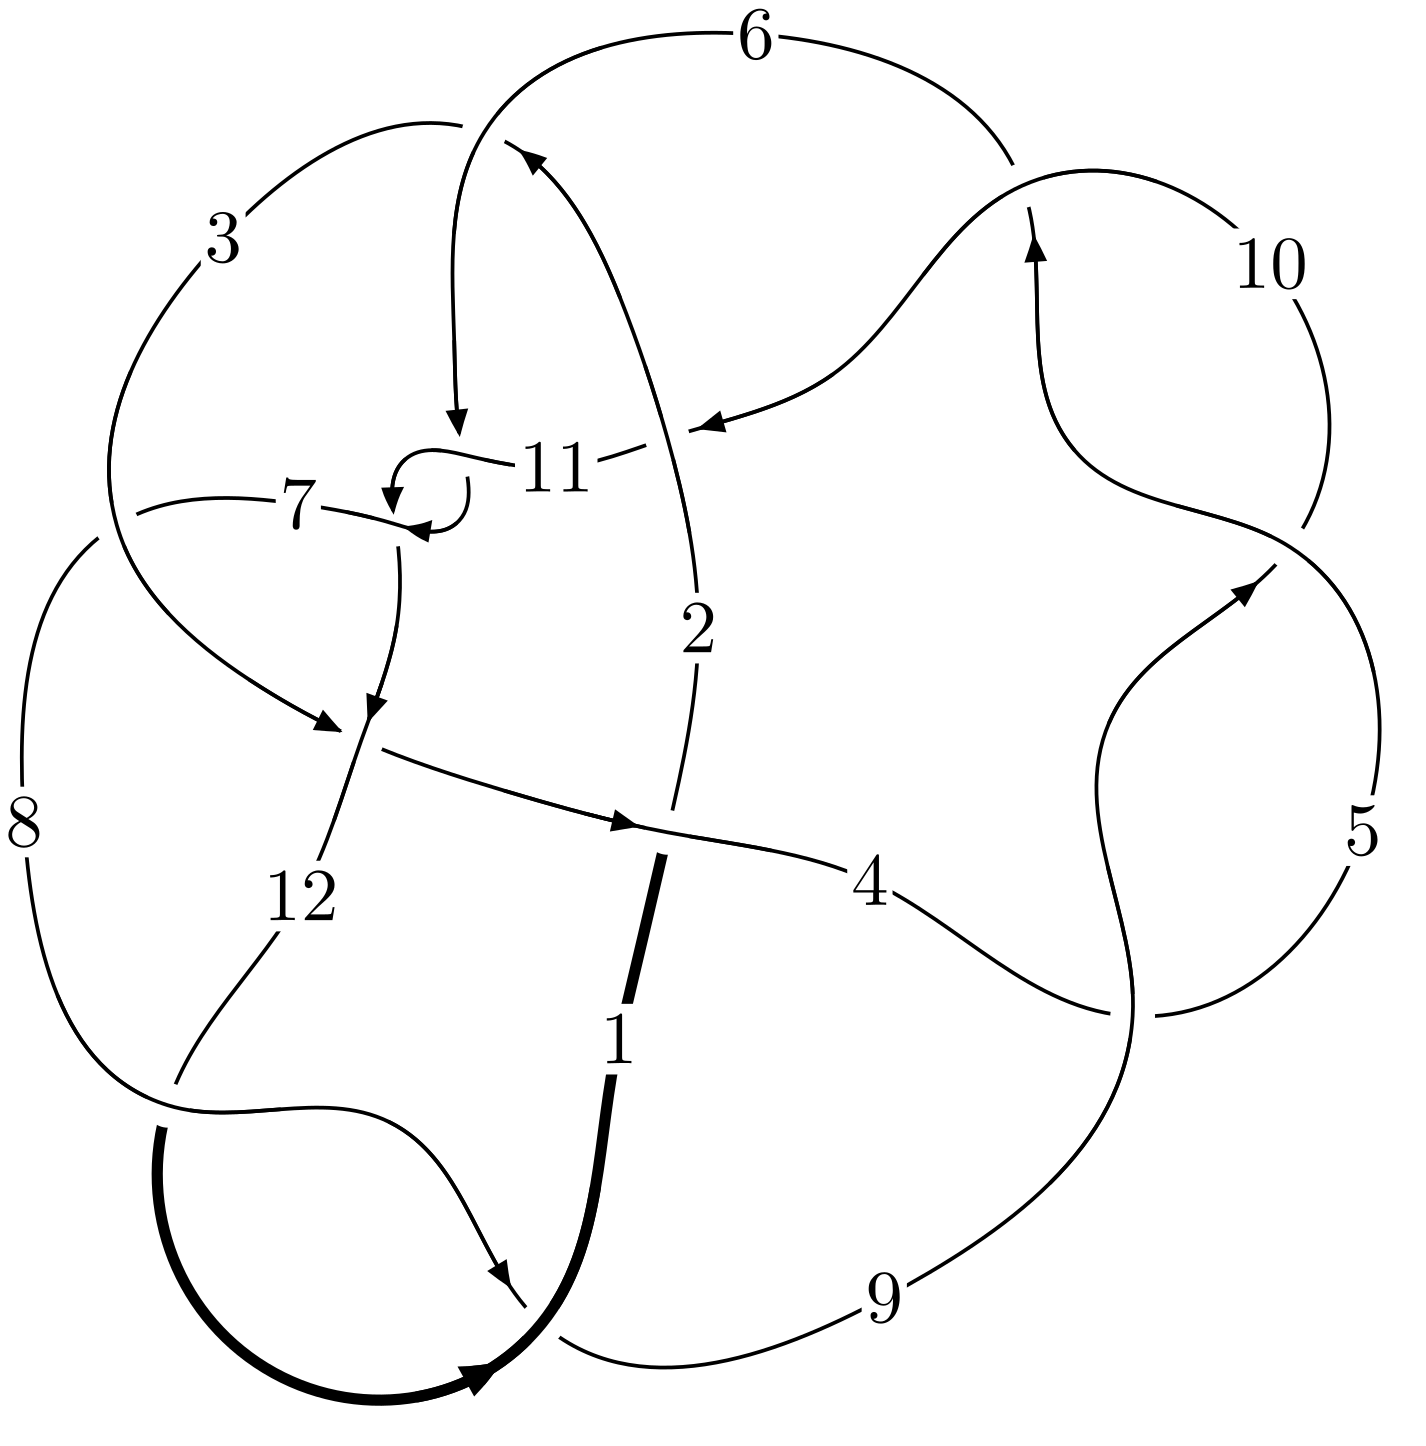
\includegraphics[width=112pt]{../../../GIT/diagram.site/Diagrams/png/1803_12a_1002.png}\\
\ \ \ A knot diagram\footnotemark}&
\allowdisplaybreaks
\textbf{Linearized knot diagam} \\
\cline{2-2}
 &
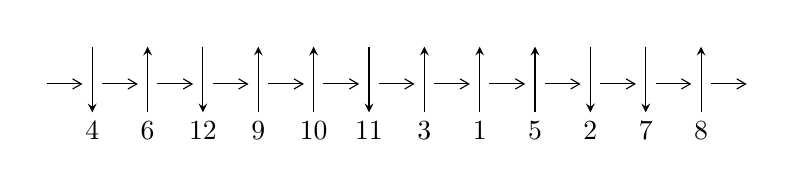
\begin{tikzpicture}[x=20pt, y=17pt]
	% nodes
	\node (C0) at (0, 0) {};
	\node (C1) at (1, 0) {};
	\node (C1U) at (1, +1) {};
	\node (C1D) at (1, -1) {4};

	\node (C2) at (2, 0) {};
	\node (C2U) at (2, +1) {};
	\node (C2D) at (2, -1) {6};

	\node (C3) at (3, 0) {};
	\node (C3U) at (3, +1) {};
	\node (C3D) at (3, -1) {12};

	\node (C4) at (4, 0) {};
	\node (C4U) at (4, +1) {};
	\node (C4D) at (4, -1) {9};

	\node (C5) at (5, 0) {};
	\node (C5U) at (5, +1) {};
	\node (C5D) at (5, -1) {10};

	\node (C6) at (6, 0) {};
	\node (C6U) at (6, +1) {};
	\node (C6D) at (6, -1) {11};

	\node (C7) at (7, 0) {};
	\node (C7U) at (7, +1) {};
	\node (C7D) at (7, -1) {3};

	\node (C8) at (8, 0) {};
	\node (C8U) at (8, +1) {};
	\node (C8D) at (8, -1) {1};

	\node (C9) at (9, 0) {};
	\node (C9U) at (9, +1) {};
	\node (C9D) at (9, -1) {5};

	\node (C10) at (10, 0) {};
	\node (C10U) at (10, +1) {};
	\node (C10D) at (10, -1) {2};

	\node (C11) at (11, 0) {};
	\node (C11U) at (11, +1) {};
	\node (C11D) at (11, -1) {7};

	\node (C12) at (12, 0) {};
	\node (C12U) at (12, +1) {};
	\node (C12D) at (12, -1) {8};
	\node (C13) at (13, 0) {};

	% arrows
	\draw[->,>={angle 60}]
	(C0) edge (C1) (C1) edge (C2) (C2) edge (C3) (C3) edge (C4) (C4) edge (C5) (C5) edge (C6) (C6) edge (C7) (C7) edge (C8) (C8) edge (C9) (C9) edge (C10) (C10) edge (C11) (C11) edge (C12) (C12) edge (C13) ;	\draw[->,>=stealth]
	(C1U) edge (C1D) (C2D) edge (C2U) (C3U) edge (C3D) (C4D) edge (C4U) (C5D) edge (C5U) (C6U) edge (C6D) (C7D) edge (C7U) (C8D) edge (C8U) (C9D) edge (C9U) (C10U) edge (C10D) (C11U) edge (C11D) (C12D) edge (C12U) ;
	\end{tikzpicture} \\
\hhline{~~} \\& 
\textbf{Solving Sequence} \\ \cline{2-2} 
 &
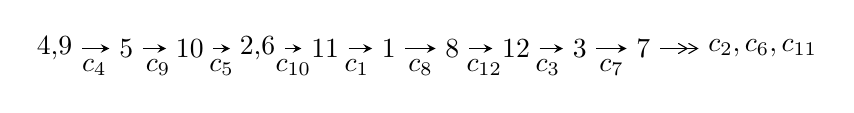
\begin{tikzpicture}[x=23pt, y=7pt]
	% node
	\node (A0) at (-1/8, 0) {4,9};
	\node (A1) at (1, 0) {5};
	\node (A2) at (2, 0) {10};
	\node (A3) at (49/16, 0) {2,6};
	\node (A4) at (33/8, 0) {11};
	\node (A5) at (41/8, 0) {1};
	\node (A6) at (49/8, 0) {8};
	\node (A7) at (57/8, 0) {12};
	\node (A8) at (65/8, 0) {3};
	\node (A9) at (73/8, 0) {7};
	\node (C1) at (1/2, -1) {$c_{4}$};
	\node (C2) at (3/2, -1) {$c_{9}$};
	\node (C3) at (5/2, -1) {$c_{5}$};
	\node (C4) at (29/8, -1) {$c_{10}$};
	\node (C5) at (37/8, -1) {$c_{1}$};
	\node (C6) at (45/8, -1) {$c_{8}$};
	\node (C7) at (53/8, -1) {$c_{12}$};
	\node (C8) at (61/8, -1) {$c_{3}$};
	\node (C9) at (69/8, -1) {$c_{7}$};
	\node (A10) at (11, 0) {$c_{2},c_{6},c_{11}$};

	% edge
	\draw[->,>=stealth]	
	(A0) edge (A1) (A1) edge (A2) (A2) edge (A3) (A3) edge (A4) (A4) edge (A5) (A5) edge (A6) (A6) edge (A7) (A7) edge (A8) (A8) edge (A9) ;
	\draw[->>,>={angle 60}]	
	(A9) edge (A10);
\end{tikzpicture} \\ 

\end{tabular} \\

\footnotetext{
The image of knot diagram is generated by the software ``\textbf{Draw programme}" developed by Andrew Bartholomew(\url{http://www.layer8.co.uk/maths/draw/index.htm\#Running-draw}), where we modified some parts for our purpose(\url{https://github.com/CATsTAILs/LinksPainter}).
}\phantom \\ \newline 
\centering \textbf{Ideals for irreducible components\footnotemark of $X_{\text{par}}$} 
 
\begin{align*}
I^u_{1}&=\langle 
1.32196\times10^{269} u^{109}-6.64912\times10^{268} u^{108}+\cdots+2.22425\times10^{269} b-9.95049\times10^{269},\\
\phantom{I^u_{1}}&\phantom{= \langle  }-1.97255\times10^{271} u^{109}+1.64430\times10^{271} u^{108}+\cdots+2.58013\times10^{271} a+1.37216\times10^{273},\\
\phantom{I^u_{1}}&\phantom{= \langle  }u^{110}-2 u^{109}+\cdots+142 u+29\rangle \\
I^u_{2}&=\langle 
-9 u^{16}+5 u^{15}+\cdots+19 b+25,\;172 u^{16}+48 u^{15}+\cdots+133 a-178,\;u^{17}- u^{16}+\cdots-2 u+1\rangle \\
I^u_{3}&=\langle 
b,\;a-1,\;u+1\rangle \\
I^u_{4}&=\langle 
b+1,\;a^3-2 a^2- a+1,\;u+1\rangle \\
\\
\end{align*}
\raggedright * 4 irreducible components of $\dim_{\mathbb{C}}=0$, with total 131 representations.\\
\footnotetext{All coefficients of polynomials are rational numbers. But the coefficients are sometimes approximated in decimal forms when there is not enough margin.}
\newpage
\renewcommand{\arraystretch}{1}
\centering \section*{I. $I^u_{1}= \langle 1.32\times10^{269} u^{109}-6.65\times10^{268} u^{108}+\cdots+2.22\times10^{269} b-9.95\times10^{269},\;-1.97\times10^{271} u^{109}+1.64\times10^{271} u^{108}+\cdots+2.58\times10^{271} a+1.37\times10^{273},\;u^{110}-2 u^{109}+\cdots+142 u+29 \rangle$}
\flushleft \textbf{(i) Arc colorings}\\
\begin{tabular}{m{7pt} m{180pt} m{7pt} m{180pt} }
\flushright $a_{4}=$&$\begin{pmatrix}1\\0\end{pmatrix}$ \\
\flushright $a_{9}=$&$\begin{pmatrix}0\\u\end{pmatrix}$ \\
\flushright $a_{5}=$&$\begin{pmatrix}1\\- u^2\end{pmatrix}$ \\
\flushright $a_{10}=$&$\begin{pmatrix}u\\- u^3+u\end{pmatrix}$ \\
\flushright $a_{2}=$&$\begin{pmatrix}0.764513 u^{109}-0.637292 u^{108}+\cdots-278.114 u-53.1817\\-0.594340 u^{109}+0.298937 u^{108}+\cdots+45.4409 u+4.47364\end{pmatrix}$ \\
\flushright $a_{6}=$&$\begin{pmatrix}- u^2+1\\u^4-2 u^2\end{pmatrix}$ \\
\flushright $a_{11}=$&$\begin{pmatrix}0.797741 u^{109}-0.903180 u^{108}+\cdots-224.858 u-15.9278\\-0.0931427 u^{109}-0.0484952 u^{108}+\cdots-31.3015 u-2.78574\end{pmatrix}$ \\
\flushright $a_{1}=$&$\begin{pmatrix}0.170173 u^{109}-0.338354 u^{108}+\cdots-232.673 u-48.7081\\-0.594340 u^{109}+0.298937 u^{108}+\cdots+45.4409 u+4.47364\end{pmatrix}$ \\
\flushright $a_{8}=$&$\begin{pmatrix}0.655043 u^{109}-1.14852 u^{108}+\cdots-381.879 u-32.5792\\0.735729 u^{109}-0.404328 u^{108}+\cdots-126.324 u-20.0634\end{pmatrix}$ \\
\flushright $a_{12}=$&$\begin{pmatrix}0.503853 u^{109}-0.796458 u^{108}+\cdots-126.933 u+0.220543\\-0.0221484 u^{109}+0.288965 u^{108}+\cdots+100.879 u+14.9464\end{pmatrix}$ \\
\flushright $a_{3}=$&$\begin{pmatrix}0.144433 u^{109}-0.268865 u^{108}+\cdots-245.630 u-49.3323\\-0.286770 u^{109}+0.0910355 u^{108}+\cdots+14.5909 u-0.821688\end{pmatrix}$ \\
\flushright $a_{7}=$&$\begin{pmatrix}0.787523 u^{109}-1.66427 u^{108}+\cdots-416.345 u-34.1907\\-0.0988489 u^{109}+0.179027 u^{108}+\cdots+52.5901 u+8.61063\end{pmatrix}$\\&\end{tabular}
\flushleft \textbf{(ii) Obstruction class $= -1$}\\~\\
\flushleft \textbf{(iii) Cusp Shapes $= -0.663649 u^{109}+1.82718 u^{108}+\cdots+495.499 u+53.9213$}\\~\\
\newpage\renewcommand{\arraystretch}{1}
\flushleft \textbf{(iv) u-Polynomials at the component}\newline \\
\begin{tabular}{m{50pt}|m{274pt}}
Crossings & \hspace{64pt}u-Polynomials at each crossing \\
\hline $$\begin{aligned}c_{1}\end{aligned}$$&$\begin{aligned}
&u^{110}+6 u^{109}+\cdots+6916672 u-1324600
\end{aligned}$\\
\hline $$\begin{aligned}c_{2}\end{aligned}$$&$\begin{aligned}
&u^{110}-8 u^{108}+\cdots-1232 u-167
\end{aligned}$\\
\hline $$\begin{aligned}c_{3}\end{aligned}$$&$\begin{aligned}
&u^{110}-3 u^{109}+\cdots-71 u+1
\end{aligned}$\\
\hline $$\begin{aligned}c_{4},c_{5},c_{9}\end{aligned}$$&$\begin{aligned}
&u^{110}+2 u^{109}+\cdots-142 u+29
\end{aligned}$\\
\hline $$\begin{aligned}c_{6},c_{11}\end{aligned}$$&$\begin{aligned}
&u^{110}-2 u^{109}+\cdots+58 u+1
\end{aligned}$\\
\hline $$\begin{aligned}c_{7}\end{aligned}$$&$\begin{aligned}
&u^{110}+u^{109}+\cdots+1532 u-40
\end{aligned}$\\
\hline $$\begin{aligned}c_{8},c_{12}\end{aligned}$$&$\begin{aligned}
&u^{110}+2 u^{109}+\cdots-455 u+73
\end{aligned}$\\
\hline $$\begin{aligned}c_{10}\end{aligned}$$&$\begin{aligned}
&u^{110}+6 u^{109}+\cdots+62 u+5
\end{aligned}$\\
\hline
\end{tabular}\\~\\
\newpage\renewcommand{\arraystretch}{1}
\flushleft \textbf{(v) Riley Polynomials at the component}\newline \\
\begin{tabular}{m{50pt}|m{274pt}}
Crossings & \hspace{64pt}Riley Polynomials at each crossing \\
\hline $$\begin{aligned}c_{1}\end{aligned}$$&$\begin{aligned}
&y^{110}+54 y^{109}+\cdots-68056508021984 y+1754565160000
\end{aligned}$\\
\hline $$\begin{aligned}c_{2}\end{aligned}$$&$\begin{aligned}
&y^{110}-16 y^{109}+\cdots-1812078 y+27889
\end{aligned}$\\
\hline $$\begin{aligned}c_{3}\end{aligned}$$&$\begin{aligned}
&y^{110}-13 y^{109}+\cdots-3915 y+1
\end{aligned}$\\
\hline $$\begin{aligned}c_{4},c_{5},c_{9}\end{aligned}$$&$\begin{aligned}
&y^{110}-122 y^{109}+\cdots-73814 y+841
\end{aligned}$\\
\hline $$\begin{aligned}c_{6},c_{11}\end{aligned}$$&$\begin{aligned}
&y^{110}-86 y^{109}+\cdots-814 y+1
\end{aligned}$\\
\hline $$\begin{aligned}c_{7}\end{aligned}$$&$\begin{aligned}
&y^{110}-5 y^{109}+\cdots-2675984 y+1600
\end{aligned}$\\
\hline $$\begin{aligned}c_{8},c_{12}\end{aligned}$$&$\begin{aligned}
&y^{110}-90 y^{109}+\cdots-177533 y+5329
\end{aligned}$\\
\hline $$\begin{aligned}c_{10}\end{aligned}$$&$\begin{aligned}
&y^{110}+114 y^{108}+\cdots-4464 y+25
\end{aligned}$\\
\hline
\end{tabular}\\~\\
\newpage\flushleft \textbf{(vi) Complex Volumes and Cusp Shapes}
$$\begin{array}{c|c|c}  
\text{Solutions to }I^u_{1}& \I (\text{vol} + \sqrt{-1}CS) & \text{Cusp shape}\\
 \hline 
\begin{aligned}
u &= -0.561117 + 0.839392 I \\
a &= -0.303990 + 0.131847 I \\
b &= -0.421456 - 1.140830 I\end{aligned}
 & \phantom{-}2.56229 - 4.55331 I & \phantom{-0.000000 } 0 \\ \hline\begin{aligned}
u &= -0.561117 - 0.839392 I \\
a &= -0.303990 - 0.131847 I \\
b &= -0.421456 + 1.140830 I\end{aligned}
 & \phantom{-}2.56229 + 4.55331 I & \phantom{-0.000000 } 0 \\ \hline\begin{aligned}
u &= -0.927916 + 0.225382 I \\
a &= \phantom{-}0.664044 - 0.078712 I \\
b &= \phantom{-}1.003900 + 0.171942 I\end{aligned}
 & \phantom{-}0.313706 + 0.175524 I & \phantom{-0.000000 } 0 \\ \hline\begin{aligned}
u &= -0.927916 - 0.225382 I \\
a &= \phantom{-}0.664044 + 0.078712 I \\
b &= \phantom{-}1.003900 - 0.171942 I\end{aligned}
 & \phantom{-}0.313706 - 0.175524 I & \phantom{-0.000000 } 0 \\ \hline\begin{aligned}
u &= \phantom{-}0.959964 + 0.457834 I \\
a &= \phantom{-}1.44411 - 0.00057 I \\
b &= -0.378698 - 0.662224 I\end{aligned}
 & \phantom{-}1.63508 - 0.94549 I & \phantom{-0.000000 } 0 \\ \hline\begin{aligned}
u &= \phantom{-}0.959964 - 0.457834 I \\
a &= \phantom{-}1.44411 + 0.00057 I \\
b &= -0.378698 + 0.662224 I\end{aligned}
 & \phantom{-}1.63508 + 0.94549 I & \phantom{-0.000000 } 0 \\ \hline\begin{aligned}
u &= -0.316258 + 1.015460 I \\
a &= -0.371801 - 0.517839 I \\
b &= \phantom{-}0.327371 - 0.681355 I\end{aligned}
 & -1.22848 + 8.07799 I & \phantom{-0.000000 } 0 \\ \hline\begin{aligned}
u &= -0.316258 - 1.015460 I \\
a &= -0.371801 + 0.517839 I \\
b &= \phantom{-}0.327371 + 0.681355 I\end{aligned}
 & -1.22848 - 8.07799 I & \phantom{-0.000000 } 0 \\ \hline\begin{aligned}
u &= \phantom{-}1.06797\phantom{ +0.000000I} \\
a &= \phantom{-}0.610464\phantom{ +0.000000I} \\
b &= -1.19855\phantom{ +0.000000I}\end{aligned}
 & \phantom{-}0.377278\phantom{ +0.000000I} & \phantom{-0.000000 } 0 \\ \hline\begin{aligned}
u &= -0.729463 + 0.787079 I \\
a &= \phantom{-}0.260649 - 0.445540 I \\
b &= \phantom{-}0.91205 + 1.10958 I\end{aligned}
 & \phantom{-}0.03302 - 13.85620 I & \phantom{-0.000000 } 0\\
 \hline 
 \end{array}$$\newpage$$\begin{array}{c|c|c}  
\text{Solutions to }I^u_{1}& \I (\text{vol} + \sqrt{-1}CS) & \text{Cusp shape}\\
 \hline 
\begin{aligned}
u &= -0.729463 - 0.787079 I \\
a &= \phantom{-}0.260649 + 0.445540 I \\
b &= \phantom{-}0.91205 - 1.10958 I\end{aligned}
 & \phantom{-}0.03302 + 13.85620 I & \phantom{-0.000000 } 0 \\ \hline\begin{aligned}
u &= -0.567089 + 0.952408 I \\
a &= \phantom{-}0.498975 + 0.089888 I \\
b &= \phantom{-}0.239021 + 0.674220 I\end{aligned}
 & \phantom{-}2.45698 - 1.04644 I & \phantom{-0.000000 } 0 \\ \hline\begin{aligned}
u &= -0.567089 - 0.952408 I \\
a &= \phantom{-}0.498975 - 0.089888 I \\
b &= \phantom{-}0.239021 - 0.674220 I\end{aligned}
 & \phantom{-}2.45698 + 1.04644 I & \phantom{-0.000000 } 0 \\ \hline\begin{aligned}
u &= \phantom{-}0.530952 + 0.713864 I \\
a &= -0.171699 + 0.282459 I \\
b &= \phantom{-}0.927780 + 0.145012 I\end{aligned}
 & -4.74837 - 4.09767 I & \phantom{-0.000000 } 0 \\ \hline\begin{aligned}
u &= \phantom{-}0.530952 - 0.713864 I \\
a &= -0.171699 - 0.282459 I \\
b &= \phantom{-}0.927780 - 0.145012 I\end{aligned}
 & -4.74837 + 4.09767 I & \phantom{-0.000000 } 0 \\ \hline\begin{aligned}
u &= \phantom{-}0.773574 + 0.809008 I \\
a &= \phantom{-}0.356404 + 0.358372 I \\
b &= \phantom{-}0.741088 - 0.968332 I\end{aligned}
 & \phantom{-}4.96862 + 8.04897 I & \phantom{-0.000000 } 0 \\ \hline\begin{aligned}
u &= \phantom{-}0.773574 - 0.809008 I \\
a &= \phantom{-}0.356404 - 0.358372 I \\
b &= \phantom{-}0.741088 + 0.968332 I\end{aligned}
 & \phantom{-}4.96862 - 8.04897 I & \phantom{-0.000000 } 0 \\ \hline\begin{aligned}
u &= \phantom{-}0.513703 + 0.684899 I \\
a &= \phantom{-}0.142348 + 1.039150 I \\
b &= \phantom{-}0.900529 - 0.488273 I\end{aligned}
 & -4.77261 + 8.77139 I & \phantom{-0.000000 } 0 \\ \hline\begin{aligned}
u &= \phantom{-}0.513703 - 0.684899 I \\
a &= \phantom{-}0.142348 - 1.039150 I \\
b &= \phantom{-}0.900529 + 0.488273 I\end{aligned}
 & -4.77261 - 8.77139 I & \phantom{-0.000000 } 0 \\ \hline\begin{aligned}
u &= -0.663764 + 0.503751 I \\
a &= \phantom{-}1.221330 + 0.082009 I \\
b &= -0.057478 + 0.823623 I\end{aligned}
 & \phantom{-}2.58165 - 0.03463 I & \phantom{-0.000000 } 0\\
 \hline 
 \end{array}$$\newpage$$\begin{array}{c|c|c}  
\text{Solutions to }I^u_{1}& \I (\text{vol} + \sqrt{-1}CS) & \text{Cusp shape}\\
 \hline 
\begin{aligned}
u &= -0.663764 - 0.503751 I \\
a &= \phantom{-}1.221330 - 0.082009 I \\
b &= -0.057478 - 0.823623 I\end{aligned}
 & \phantom{-}2.58165 + 0.03463 I & \phantom{-0.000000 } 0 \\ \hline\begin{aligned}
u &= -1.18213\phantom{ +0.000000I} \\
a &= \phantom{-}1.50672\phantom{ +0.000000I} \\
b &= -1.65419\phantom{ +0.000000I}\end{aligned}
 & -2.89730\phantom{ +0.000000I} & \phantom{-0.000000 } 0 \\ \hline\begin{aligned}
u &= \phantom{-}0.586598 + 0.524605 I \\
a &= -0.292439 - 0.789688 I \\
b &= -0.91004 + 1.31036 I\end{aligned}
 & -2.19521 + 5.10239 I & \phantom{-0.000000 } 0 \\ \hline\begin{aligned}
u &= \phantom{-}0.586598 - 0.524605 I \\
a &= -0.292439 + 0.789688 I \\
b &= -0.91004 - 1.31036 I\end{aligned}
 & -2.19521 - 5.10239 I & \phantom{-0.000000 } 0 \\ \hline\begin{aligned}
u &= -0.467339 + 0.592282 I \\
a &= -0.569458 + 0.168185 I \\
b &= -0.665733 - 1.241350 I\end{aligned}
 & \phantom{-}2.02732 - 3.98332 I & \phantom{-0.000000 } 0 \\ \hline\begin{aligned}
u &= -0.467339 - 0.592282 I \\
a &= -0.569458 - 0.168185 I \\
b &= -0.665733 + 1.241350 I\end{aligned}
 & \phantom{-}2.02732 + 3.98332 I & \phantom{-0.000000 } 0 \\ \hline\begin{aligned}
u &= -0.388667 + 0.644207 I \\
a &= \phantom{-}0.609698 - 0.868649 I \\
b &= \phantom{-}0.610278 + 0.381243 I\end{aligned}
 & \phantom{-}0.34111 - 3.17260 I & \phantom{-0.000000 } 0 \\ \hline\begin{aligned}
u &= -0.388667 - 0.644207 I \\
a &= \phantom{-}0.609698 + 0.868649 I \\
b &= \phantom{-}0.610278 - 0.381243 I\end{aligned}
 & \phantom{-}0.34111 + 3.17260 I & \phantom{-0.000000 } 0 \\ \hline\begin{aligned}
u &= -1.259520 + 0.213847 I \\
a &= \phantom{-}0.457879 - 0.631771 I \\
b &= \phantom{-}0.247105 + 0.397332 I\end{aligned}
 & \phantom{-}1.79921 - 0.26763 I & \phantom{-0.000000 } 0 \\ \hline\begin{aligned}
u &= -1.259520 - 0.213847 I \\
a &= \phantom{-}0.457879 + 0.631771 I \\
b &= \phantom{-}0.247105 - 0.397332 I\end{aligned}
 & \phantom{-}1.79921 + 0.26763 I & \phantom{-0.000000 } 0\\
 \hline 
 \end{array}$$\newpage$$\begin{array}{c|c|c}  
\text{Solutions to }I^u_{1}& \I (\text{vol} + \sqrt{-1}CS) & \text{Cusp shape}\\
 \hline 
\begin{aligned}
u &= -0.705578\phantom{ +0.000000I} \\
a &= \phantom{-}0.686211\phantom{ +0.000000I} \\
b &= -1.81071\phantom{ +0.000000I}\end{aligned}
 & -4.29507\phantom{ +0.000000I} & \phantom{-0.000000 } 0 \\ \hline\begin{aligned}
u &= \phantom{-}0.197875 + 0.654372 I \\
a &= -0.167494 + 0.382578 I \\
b &= -0.76633 + 1.33681 I\end{aligned}
 & -0.64558 + 4.99505 I & \phantom{-0.000000 } 0 \\ \hline\begin{aligned}
u &= \phantom{-}0.197875 - 0.654372 I \\
a &= -0.167494 - 0.382578 I \\
b &= -0.76633 - 1.33681 I\end{aligned}
 & -0.64558 - 4.99505 I & \phantom{-0.000000 } 0 \\ \hline\begin{aligned}
u &= -0.522290 + 0.434471 I \\
a &= \phantom{-}0.191918 + 0.244207 I \\
b &= \phantom{-}0.240332 - 0.360798 I\end{aligned}
 & \phantom{-}1.176650 - 0.617251 I & \phantom{-0.000000 } 0 \\ \hline\begin{aligned}
u &= -0.522290 - 0.434471 I \\
a &= \phantom{-}0.191918 - 0.244207 I \\
b &= \phantom{-}0.240332 + 0.360798 I\end{aligned}
 & \phantom{-}1.176650 + 0.617251 I & \phantom{-0.000000 } 0 \\ \hline\begin{aligned}
u &= -0.553619 + 0.372557 I \\
a &= \phantom{-}0.96752 + 1.55292 I \\
b &= -1.005840 - 0.395070 I\end{aligned}
 & -3.87784 - 1.19491 I & \phantom{-0.000000 -}0. + 3.34499 I \\ \hline\begin{aligned}
u &= -0.553619 - 0.372557 I \\
a &= \phantom{-}0.96752 - 1.55292 I \\
b &= -1.005840 + 0.395070 I\end{aligned}
 & -3.87784 + 1.19491 I & \phantom{-0.000000 } 0. - 3.34499 I \\ \hline\begin{aligned}
u &= -0.609765 + 0.259275 I \\
a &= -1.74801 + 1.21596 I \\
b &= -0.304239 - 1.351150 I\end{aligned}
 & \phantom{-}2.09953 - 6.85443 I & \phantom{-}6.48042 + 7.99330 I \\ \hline\begin{aligned}
u &= -0.609765 - 0.259275 I \\
a &= -1.74801 - 1.21596 I \\
b &= -0.304239 + 1.351150 I\end{aligned}
 & \phantom{-}2.09953 + 6.85443 I & \phantom{-}6.48042 - 7.99330 I \\ \hline\begin{aligned}
u &= \phantom{-}1.345720 + 0.087315 I \\
a &= \phantom{-}0.62240 - 1.65565 I \\
b &= -0.800525 + 1.105590 I\end{aligned}
 & -0.36834 + 3.75700 I & \phantom{-0.000000 } 0\\
 \hline 
 \end{array}$$\newpage$$\begin{array}{c|c|c}  
\text{Solutions to }I^u_{1}& \I (\text{vol} + \sqrt{-1}CS) & \text{Cusp shape}\\
 \hline 
\begin{aligned}
u &= \phantom{-}1.345720 - 0.087315 I \\
a &= \phantom{-}0.62240 + 1.65565 I \\
b &= -0.800525 - 1.105590 I\end{aligned}
 & -0.36834 - 3.75700 I & \phantom{-0.000000 } 0 \\ \hline\begin{aligned}
u &= \phantom{-}0.338412 + 0.532311 I \\
a &= \phantom{-}1.049160 - 0.832600 I \\
b &= -0.652477 - 0.520997 I\end{aligned}
 & -2.89784 - 1.43811 I & -1.19470 + 1.30013 I \\ \hline\begin{aligned}
u &= \phantom{-}0.338412 - 0.532311 I \\
a &= \phantom{-}1.049160 + 0.832600 I \\
b &= -0.652477 + 0.520997 I\end{aligned}
 & -2.89784 + 1.43811 I & -1.19470 - 1.30013 I \\ \hline\begin{aligned}
u &= \phantom{-}0.384390 + 0.472117 I \\
a &= -0.057955 - 0.709801 I \\
b &= -0.072193 + 1.060730 I\end{aligned}
 & -1.80335 + 4.26864 I & \phantom{-0.000000 } 0. - 8.46446 I \\ \hline\begin{aligned}
u &= \phantom{-}0.384390 - 0.472117 I \\
a &= -0.057955 + 0.709801 I \\
b &= -0.072193 - 1.060730 I\end{aligned}
 & -1.80335 - 4.26864 I & \phantom{-0.000000 -}0. + 8.46446 I \\ \hline\begin{aligned}
u &= -1.43088 + 0.15235 I \\
a &= \phantom{-}0.25860 + 2.38251 I \\
b &= -1.22902 - 2.26534 I\end{aligned}
 & \phantom{-}4.56457 - 7.63869 I & \phantom{-0.000000 } 0 \\ \hline\begin{aligned}
u &= -1.43088 - 0.15235 I \\
a &= \phantom{-}0.25860 - 2.38251 I \\
b &= -1.22902 + 2.26534 I\end{aligned}
 & \phantom{-}4.56457 + 7.63869 I & \phantom{-0.000000 } 0 \\ \hline\begin{aligned}
u &= -0.191657 + 0.512923 I \\
a &= -0.046361 + 0.638848 I \\
b &= -1.112870 - 0.427835 I\end{aligned}
 & -5.06856 - 1.65720 I & -7.16569 + 4.46058 I \\ \hline\begin{aligned}
u &= -0.191657 - 0.512923 I \\
a &= -0.046361 - 0.638848 I \\
b &= -1.112870 + 0.427835 I\end{aligned}
 & -5.06856 + 1.65720 I & -7.16569 - 4.46058 I \\ \hline\begin{aligned}
u &= \phantom{-}1.46115 + 0.08625 I \\
a &= -0.37508 + 1.49521 I \\
b &= -0.279736 - 0.529528 I\end{aligned}
 & \phantom{-}3.59759 + 4.20792 I & \phantom{-0.000000 } 0\\
 \hline 
 \end{array}$$\newpage$$\begin{array}{c|c|c}  
\text{Solutions to }I^u_{1}& \I (\text{vol} + \sqrt{-1}CS) & \text{Cusp shape}\\
 \hline 
\begin{aligned}
u &= \phantom{-}1.46115 - 0.08625 I \\
a &= -0.37508 - 1.49521 I \\
b &= -0.279736 + 0.529528 I\end{aligned}
 & \phantom{-}3.59759 - 4.20792 I & \phantom{-0.000000 } 0 \\ \hline\begin{aligned}
u &= \phantom{-}1.46767\phantom{ +0.000000I} \\
a &= \phantom{-}0.691382\phantom{ +0.000000I} \\
b &= -1.86135\phantom{ +0.000000I}\end{aligned}
 & \phantom{-}4.07909\phantom{ +0.000000I} & \phantom{-0.000000 } 0 \\ \hline\begin{aligned}
u &= -1.46887 + 0.01504 I \\
a &= \phantom{-}0.25445 - 1.71637 I \\
b &= -0.311834 + 0.911854 I\end{aligned}
 & \phantom{-}4.77660 + 1.78089 I & \phantom{-0.000000 } 0 \\ \hline\begin{aligned}
u &= -1.46887 - 0.01504 I \\
a &= \phantom{-}0.25445 + 1.71637 I \\
b &= -0.311834 - 0.911854 I\end{aligned}
 & \phantom{-}4.77660 - 1.78089 I & \phantom{-0.000000 } 0 \\ \hline\begin{aligned}
u &= \phantom{-}1.48030 + 0.19076 I \\
a &= -0.00626 + 1.52329 I \\
b &= \phantom{-}0.500378 - 0.750683 I\end{aligned}
 & \phantom{-}6.44612 + 6.13114 I & \phantom{-0.000000 } 0 \\ \hline\begin{aligned}
u &= \phantom{-}1.48030 - 0.19076 I \\
a &= -0.00626 - 1.52329 I \\
b &= \phantom{-}0.500378 + 0.750683 I\end{aligned}
 & \phantom{-}6.44612 - 6.13114 I & \phantom{-0.000000 } 0 \\ \hline\begin{aligned}
u &= \phantom{-}0.498224 + 0.071301 I \\
a &= \phantom{-}1.59392 + 0.46947 I \\
b &= \phantom{-}0.764381 - 1.087900 I\end{aligned}
 & \phantom{-}4.99636 - 2.04697 I & \phantom{-}13.62932 + 3.40547 I \\ \hline\begin{aligned}
u &= \phantom{-}0.498224 - 0.071301 I \\
a &= \phantom{-}1.59392 - 0.46947 I \\
b &= \phantom{-}0.764381 + 1.087900 I\end{aligned}
 & \phantom{-}4.99636 + 2.04697 I & \phantom{-}13.62932 - 3.40547 I \\ \hline\begin{aligned}
u &= -1.49656 + 0.05118 I \\
a &= \phantom{-}0.44142 + 1.68291 I \\
b &= -0.376738 - 1.055420 I\end{aligned}
 & \phantom{-}4.71699 - 2.04167 I & \phantom{-0.000000 } 0 \\ \hline\begin{aligned}
u &= -1.49656 - 0.05118 I \\
a &= \phantom{-}0.44142 - 1.68291 I \\
b &= -0.376738 + 1.055420 I\end{aligned}
 & \phantom{-}4.71699 + 2.04167 I & \phantom{-0.000000 } 0\\
 \hline 
 \end{array}$$\newpage$$\begin{array}{c|c|c}  
\text{Solutions to }I^u_{1}& \I (\text{vol} + \sqrt{-1}CS) & \text{Cusp shape}\\
 \hline 
\begin{aligned}
u &= -1.49200 + 0.15868 I \\
a &= -0.31177 + 1.83486 I \\
b &= \phantom{-}0.11957 - 1.60278 I\end{aligned}
 & \phantom{-}4.41842 - 6.58737 I & \phantom{-0.000000 } 0 \\ \hline\begin{aligned}
u &= -1.49200 - 0.15868 I \\
a &= -0.31177 - 1.83486 I \\
b &= \phantom{-}0.11957 + 1.60278 I\end{aligned}
 & \phantom{-}4.41842 + 6.58737 I & \phantom{-0.000000 } 0 \\ \hline\begin{aligned}
u &= \phantom{-}1.51008 + 0.00548 I \\
a &= -0.76849 + 2.42077 I \\
b &= \phantom{-}1.57911 - 2.38327 I\end{aligned}
 & \phantom{-}7.37201 - 5.32957 I & \phantom{-0.000000 } 0 \\ \hline\begin{aligned}
u &= \phantom{-}1.51008 - 0.00548 I \\
a &= -0.76849 - 2.42077 I \\
b &= \phantom{-}1.57911 + 2.38327 I\end{aligned}
 & \phantom{-}7.37201 + 5.32957 I & \phantom{-0.000000 } 0 \\ \hline\begin{aligned}
u &= -1.52187 + 0.03609 I \\
a &= -0.105944 + 1.408030 I \\
b &= -0.98553 - 1.09051 I\end{aligned}
 & \phantom{-}11.45720 - 3.34903 I & \phantom{-0.000000 } 0 \\ \hline\begin{aligned}
u &= -1.52187 - 0.03609 I \\
a &= -0.105944 - 1.408030 I \\
b &= -0.98553 + 1.09051 I\end{aligned}
 & \phantom{-}11.45720 + 3.34903 I & \phantom{-0.000000 } 0 \\ \hline\begin{aligned}
u &= \phantom{-}1.51607 + 0.14680 I \\
a &= -0.307512 - 1.226570 I \\
b &= \phantom{-}0.284687 + 1.072820 I\end{aligned}
 & \phantom{-}7.84229 + 2.83049 I & \phantom{-0.000000 } 0 \\ \hline\begin{aligned}
u &= \phantom{-}1.51607 - 0.14680 I \\
a &= -0.307512 + 1.226570 I \\
b &= \phantom{-}0.284687 - 1.072820 I\end{aligned}
 & \phantom{-}7.84229 - 2.83049 I & \phantom{-0.000000 } 0 \\ \hline\begin{aligned}
u &= \phantom{-}1.52317 + 0.16202 I \\
a &= \phantom{-}0.19102 - 2.07830 I \\
b &= -1.06013 + 1.93180 I\end{aligned}
 & \phantom{-}8.63374 + 6.61963 I & \phantom{-0.000000 } 0 \\ \hline\begin{aligned}
u &= \phantom{-}1.52317 - 0.16202 I \\
a &= \phantom{-}0.19102 + 2.07830 I \\
b &= -1.06013 - 1.93180 I\end{aligned}
 & \phantom{-}8.63374 - 6.61963 I & \phantom{-0.000000 } 0\\
 \hline 
 \end{array}$$\newpage$$\begin{array}{c|c|c}  
\text{Solutions to }I^u_{1}& \I (\text{vol} + \sqrt{-1}CS) & \text{Cusp shape}\\
 \hline 
\begin{aligned}
u &= -1.52037 + 0.21522 I \\
a &= -0.32083 - 1.59097 I \\
b &= \phantom{-}0.669087 + 0.872290 I\end{aligned}
 & \phantom{-}1.89051 - 12.02380 I & \phantom{-0.000000 } 0 \\ \hline\begin{aligned}
u &= -1.52037 - 0.21522 I \\
a &= -0.32083 + 1.59097 I \\
b &= \phantom{-}0.669087 - 0.872290 I\end{aligned}
 & \phantom{-}1.89051 + 12.02380 I & \phantom{-0.000000 } 0 \\ \hline\begin{aligned}
u &= -1.53845 + 0.01503 I \\
a &= -0.77655 - 1.50959 I \\
b &= \phantom{-}1.62064 + 1.47082 I\end{aligned}
 & \phantom{-}11.94240 + 1.77338 I & \phantom{-0.000000 } 0 \\ \hline\begin{aligned}
u &= -1.53845 - 0.01503 I \\
a &= -0.77655 + 1.50959 I \\
b &= \phantom{-}1.62064 - 1.47082 I\end{aligned}
 & \phantom{-}11.94240 - 1.77338 I & \phantom{-0.000000 } 0 \\ \hline\begin{aligned}
u &= \phantom{-}0.439368 + 0.125267 I \\
a &= -2.91173 - 0.94485 I \\
b &= -0.296311 + 0.914392 I\end{aligned}
 & \phantom{-}4.78298 + 2.77580 I & \phantom{-}10.74262 - 4.23324 I \\ \hline\begin{aligned}
u &= \phantom{-}0.439368 - 0.125267 I \\
a &= -2.91173 + 0.94485 I \\
b &= -0.296311 - 0.914392 I\end{aligned}
 & \phantom{-}4.78298 - 2.77580 I & \phantom{-}10.74262 + 4.23324 I \\ \hline\begin{aligned}
u &= \phantom{-}1.54191 + 0.10236 I \\
a &= \phantom{-}0.82257 - 1.60996 I \\
b &= -0.538138 + 1.028000 I\end{aligned}
 & \phantom{-}3.13802 + 2.89810 I & \phantom{-0.000000 } 0 \\ \hline\begin{aligned}
u &= \phantom{-}1.54191 - 0.10236 I \\
a &= \phantom{-}0.82257 + 1.60996 I \\
b &= -0.538138 - 1.028000 I\end{aligned}
 & \phantom{-}3.13802 - 2.89810 I & \phantom{-0.000000 } 0 \\ \hline\begin{aligned}
u &= -1.55010\phantom{ +0.000000I} \\
a &= \phantom{-}0.515231\phantom{ +0.000000I} \\
b &= -0.188672\phantom{ +0.000000I}\end{aligned}
 & \phantom{-}2.86877\phantom{ +0.000000I} & \phantom{-0.000000 } 0 \\ \hline\begin{aligned}
u &= \phantom{-}0.314782 + 0.316499 I \\
a &= \phantom{-}0.04286 - 1.45370 I \\
b &= -0.719949 + 0.376921 I\end{aligned}
 & -1.29001 + 0.97335 I & -5.23681 - 1.57208 I\\
 \hline 
 \end{array}$$\newpage$$\begin{array}{c|c|c}  
\text{Solutions to }I^u_{1}& \I (\text{vol} + \sqrt{-1}CS) & \text{Cusp shape}\\
 \hline 
\begin{aligned}
u &= \phantom{-}0.314782 - 0.316499 I \\
a &= \phantom{-}0.04286 + 1.45370 I \\
b &= -0.719949 - 0.376921 I\end{aligned}
 & -1.29001 - 0.97335 I & -5.23681 + 1.57208 I \\ \hline\begin{aligned}
u &= \phantom{-}1.55565 + 0.07957 I \\
a &= -0.13471 - 1.87630 I \\
b &= -0.81156 + 1.54843 I\end{aligned}
 & \phantom{-}9.40554 + 8.12188 I & \phantom{-0.000000 } 0 \\ \hline\begin{aligned}
u &= \phantom{-}1.55565 - 0.07957 I \\
a &= -0.13471 + 1.87630 I \\
b &= -0.81156 - 1.54843 I\end{aligned}
 & \phantom{-}9.40554 - 8.12188 I & \phantom{-0.000000 } 0 \\ \hline\begin{aligned}
u &= \phantom{-}1.55716 + 0.08388 I \\
a &= \phantom{-}0.079050 + 1.135280 I \\
b &= \phantom{-}0.812119 - 1.044250 I\end{aligned}
 & \phantom{-}10.06430 + 1.82526 I & \phantom{-0.000000 } 0 \\ \hline\begin{aligned}
u &= \phantom{-}1.55716 - 0.08388 I \\
a &= \phantom{-}0.079050 - 1.135280 I \\
b &= \phantom{-}0.812119 + 1.044250 I\end{aligned}
 & \phantom{-}10.06430 - 1.82526 I & \phantom{-0.000000 } 0 \\ \hline\begin{aligned}
u &= \phantom{-}0.417614 + 0.127707 I \\
a &= \phantom{-}1.22900 + 2.26831 I \\
b &= -0.244550 - 0.614686 I\end{aligned}
 & -1.42070 - 2.02385 I & \phantom{-}5.86521 + 0.25795 I \\ \hline\begin{aligned}
u &= \phantom{-}0.417614 - 0.127707 I \\
a &= \phantom{-}1.22900 - 2.26831 I \\
b &= -0.244550 + 0.614686 I\end{aligned}
 & -1.42070 + 2.02385 I & \phantom{-}5.86521 - 0.25795 I \\ \hline\begin{aligned}
u &= -0.188293 + 0.392923 I \\
a &= \phantom{-}0.53118 - 3.05353 I \\
b &= \phantom{-}0.240285 - 0.019161 I\end{aligned}
 & -1.97408 - 2.72746 I & -13.6098 + 7.1286 I \\ \hline\begin{aligned}
u &= -0.188293 - 0.392923 I \\
a &= \phantom{-}0.53118 + 3.05353 I \\
b &= \phantom{-}0.240285 + 0.019161 I\end{aligned}
 & -1.97408 + 2.72746 I & -13.6098 - 7.1286 I \\ \hline\begin{aligned}
u &= -1.56070 + 0.15405 I \\
a &= \phantom{-}0.36566 + 2.37618 I \\
b &= -1.08051 - 2.20286 I\end{aligned}
 & \phantom{-}4.99912 - 7.57034 I & \phantom{-0.000000 } 0\\
 \hline 
 \end{array}$$\newpage$$\begin{array}{c|c|c}  
\text{Solutions to }I^u_{1}& \I (\text{vol} + \sqrt{-1}CS) & \text{Cusp shape}\\
 \hline 
\begin{aligned}
u &= -1.56070 - 0.15405 I \\
a &= \phantom{-}0.36566 - 2.37618 I \\
b &= -1.08051 + 2.20286 I\end{aligned}
 & \phantom{-}4.99912 + 7.57034 I & \phantom{-0.000000 } 0 \\ \hline\begin{aligned}
u &= \phantom{-}1.57068 + 0.29738 I \\
a &= -0.14027 - 1.56575 I \\
b &= -0.71535 + 1.61442 I\end{aligned}
 & \phantom{-}9.53813 + 8.77828 I & \phantom{-0.000000 } 0 \\ \hline\begin{aligned}
u &= \phantom{-}1.57068 - 0.29738 I \\
a &= -0.14027 + 1.56575 I \\
b &= -0.71535 - 1.61442 I\end{aligned}
 & \phantom{-}9.53813 - 8.77828 I & \phantom{-0.000000 } 0 \\ \hline\begin{aligned}
u &= \phantom{-}1.60561\phantom{ +0.000000I} \\
a &= -1.37001\phantom{ +0.000000I} \\
b &= \phantom{-}2.25122\phantom{ +0.000000I}\end{aligned}
 & \phantom{-}8.86339\phantom{ +0.000000I} & \phantom{-0.000000 } 0 \\ \hline\begin{aligned}
u &= \phantom{-}0.99962 + 1.25672 I \\
a &= -0.151543 + 0.000614 I \\
b &= -0.235450 + 0.608818 I\end{aligned}
 & \phantom{-}3.59740 - 1.02869 I & \phantom{-0.000000 } 0 \\ \hline\begin{aligned}
u &= \phantom{-}0.99962 - 1.25672 I \\
a &= -0.151543 - 0.000614 I \\
b &= -0.235450 - 0.608818 I\end{aligned}
 & \phantom{-}3.59740 + 1.02869 I & \phantom{-0.000000 } 0 \\ \hline\begin{aligned}
u &= \phantom{-}1.59888 + 0.26921 I \\
a &= -0.033918 + 1.188430 I \\
b &= \phantom{-}1.01703 - 1.06081 I\end{aligned}
 & \phantom{-}9.89750 + 5.36352 I & \phantom{-0.000000 } 0 \\ \hline\begin{aligned}
u &= \phantom{-}1.59888 - 0.26921 I \\
a &= -0.033918 - 1.188430 I \\
b &= \phantom{-}1.01703 + 1.06081 I\end{aligned}
 & \phantom{-}9.89750 - 5.36352 I & \phantom{-0.000000 } 0 \\ \hline\begin{aligned}
u &= -1.63257\phantom{ +0.000000I} \\
a &= \phantom{-}0.100653\phantom{ +0.000000I} \\
b &= \phantom{-}0.830742\phantom{ +0.000000I}\end{aligned}
 & \phantom{-}10.9931\phantom{ +0.000000I} & \phantom{-0.000000 } 0 \\ \hline\begin{aligned}
u &= \phantom{-}1.61310 + 0.25881 I \\
a &= -0.30620 + 1.75307 I \\
b &= \phantom{-}1.26003 - 1.61640 I\end{aligned}
 & \phantom{-}7.7665 + 17.7910 I & \phantom{-0.000000 } 0\\
 \hline 
 \end{array}$$\newpage$$\begin{array}{c|c|c}  
\text{Solutions to }I^u_{1}& \I (\text{vol} + \sqrt{-1}CS) & \text{Cusp shape}\\
 \hline 
\begin{aligned}
u &= \phantom{-}1.61310 - 0.25881 I \\
a &= -0.30620 - 1.75307 I \\
b &= \phantom{-}1.26003 + 1.61640 I\end{aligned}
 & \phantom{-}7.7665 - 17.7910 I & \phantom{-0.000000 } 0 \\ \hline\begin{aligned}
u &= -1.61784 + 0.25740 I \\
a &= -0.18698 - 1.54451 I \\
b &= \phantom{-}1.15091 + 1.41429 I\end{aligned}
 & \phantom{-}12.8283 - 12.0395 I & \phantom{-0.000000 } 0 \\ \hline\begin{aligned}
u &= -1.61784 - 0.25740 I \\
a &= -0.18698 + 1.54451 I \\
b &= \phantom{-}1.15091 - 1.41429 I\end{aligned}
 & \phantom{-}12.8283 + 12.0395 I & \phantom{-0.000000 } 0 \\ \hline\begin{aligned}
u &= -0.341173 + 0.081513 I \\
a &= \phantom{-}2.56530 - 0.70164 I \\
b &= \phantom{-}0.63053 + 1.90328 I\end{aligned}
 & \phantom{-}0.98612 + 5.53424 I & \phantom{-}9.21361 - 3.89205 I \\ \hline\begin{aligned}
u &= -0.341173 - 0.081513 I \\
a &= \phantom{-}2.56530 + 0.70164 I \\
b &= \phantom{-}0.63053 - 1.90328 I\end{aligned}
 & \phantom{-}0.98612 - 5.53424 I & \phantom{-}9.21361 + 3.89205 I \\ \hline\begin{aligned}
u &= -1.66219 + 0.28544 I \\
a &= \phantom{-}0.105978 + 1.138680 I \\
b &= -0.87100 - 1.21409 I\end{aligned}
 & \phantom{-}11.98830 - 4.05097 I & \phantom{-0.000000 } 0 \\ \hline\begin{aligned}
u &= -1.66219 - 0.28544 I \\
a &= \phantom{-}0.105978 - 1.138680 I \\
b &= -0.87100 + 1.21409 I\end{aligned}
 & \phantom{-}11.98830 + 4.05097 I & \phantom{-0.000000 } 0 \\ \hline\begin{aligned}
u &= \phantom{-}1.83473\phantom{ +0.000000I} \\
a &= \phantom{-}0.791840\phantom{ +0.000000I} \\
b &= -1.43197\phantom{ +0.000000I}\end{aligned}
 & \phantom{-}5.03924\phantom{ +0.000000I} & \phantom{-0.000000 } 0 \\ \hline\begin{aligned}
u &= -0.159152\phantom{ +0.000000I} \\
a &= -8.05301\phantom{ +0.000000I} \\
b &= -1.10930\phantom{ +0.000000I}\end{aligned}
 & -1.59084\phantom{ +0.000000I} & -6.53800\phantom{ +0.000000I} \\ \hline\begin{aligned}
u &= -2.00901\phantom{ +0.000000I} \\
a &= -0.107919\phantom{ +0.000000I} \\
b &= \phantom{-}0.383709\phantom{ +0.000000I}\end{aligned}
 & \phantom{-}2.58600\phantom{ +0.000000I} & \phantom{-0.000000 } 0\\
 \hline 
 \end{array}$$\newpage\newpage\renewcommand{\arraystretch}{1}
\centering \section*{II. $I^u_{2}= \langle -9 u^{16}+5 u^{15}+\cdots+19 b+25,\;172 u^{16}+48 u^{15}+\cdots+133 a-178,\;u^{17}- u^{16}+\cdots-2 u+1 \rangle$}
\flushleft \textbf{(i) Arc colorings}\\
\begin{tabular}{m{7pt} m{180pt} m{7pt} m{180pt} }
\flushright $a_{4}=$&$\begin{pmatrix}1\\0\end{pmatrix}$ \\
\flushright $a_{9}=$&$\begin{pmatrix}0\\u\end{pmatrix}$ \\
\flushright $a_{5}=$&$\begin{pmatrix}1\\- u^2\end{pmatrix}$ \\
\flushright $a_{10}=$&$\begin{pmatrix}u\\- u^3+u\end{pmatrix}$ \\
\flushright $a_{2}=$&$\begin{pmatrix}-1.29323 u^{16}-0.360902 u^{15}+\cdots+5.40602 u+1.33835\\0.473684 u^{16}-0.263158 u^{15}+\cdots-0.578947 u-1.31579\end{pmatrix}$ \\
\flushright $a_{6}=$&$\begin{pmatrix}- u^2+1\\u^4-2 u^2\end{pmatrix}$ \\
\flushright $a_{11}=$&$\begin{pmatrix}-0.924812 u^{16}-0.676692 u^{15}+\cdots+5.51128 u-3.24060\\0.263158 u^{16}+0.631579 u^{15}+\cdots+0.789474 u+1.15789\end{pmatrix}$ \\
\flushright $a_{1}=$&$\begin{pmatrix}-0.819549 u^{16}-0.624060 u^{15}+\cdots+4.82707 u+0.0225564\\0.473684 u^{16}-0.263158 u^{15}+\cdots-0.578947 u-1.31579\end{pmatrix}$ \\
\flushright $a_{8}=$&$\begin{pmatrix}-0.120301 u^{16}+0.0827068 u^{15}+\cdots+4.78195 u-2.01504\\-0.390977 u^{16}-0.481203 u^{15}+\cdots+0.541353 u+0.451128\end{pmatrix}$ \\
\flushright $a_{12}=$&$\begin{pmatrix}-0.353383 u^{16}-0.819549 u^{15}+\cdots+3.79699 u+1.33083\\0.112782 u^{16}-0.0150376 u^{15}+\cdots-1.23308 u-0.360902\end{pmatrix}$ \\
\flushright $a_{3}=$&$\begin{pmatrix}-0.819549 u^{16}-0.624060 u^{15}+\cdots+4.82707 u+1.02256\\-0.0751880 u^{16}-0.323308 u^{15}+\cdots-0.511278 u-0.759398\end{pmatrix}$ \\
\flushright $a_{7}=$&$\begin{pmatrix}\frac{8}{7} u^{16}+\frac{5}{7} u^{15}+\cdots+\frac{46}{7} u-\frac{34}{7}\\-1.65414 u^{16}-0.112782 u^{15}+\cdots-0.248120 u+3.29323\end{pmatrix}$\\&\end{tabular}
\flushleft \textbf{(ii) Obstruction class $= 1$}\\~\\
\flushleft \textbf{(iii) Cusp Shapes $= \frac{47}{19} u^{16}-\frac{81}{19} u^{15}+\cdots-\frac{49}{19} u-\frac{63}{19}$}\\~\\
\newpage\renewcommand{\arraystretch}{1}
\flushleft \textbf{(iv) u-Polynomials at the component}\newline \\
\begin{tabular}{m{50pt}|m{274pt}}
Crossings & \hspace{64pt}u-Polynomials at each crossing \\
\hline $$\begin{aligned}c_{1}\end{aligned}$$&$\begin{aligned}
&u^{17}-6 u^{16}+\cdots-44 u+8
\end{aligned}$\\
\hline $$\begin{aligned}c_{2}\end{aligned}$$&$\begin{aligned}
&u^{17}-2 u^{16}+\cdots-8 u+1
\end{aligned}$\\
\hline $$\begin{aligned}c_{3}\end{aligned}$$&$\begin{aligned}
&u^{17}-2 u^{15}+\cdots-4 u-1
\end{aligned}$\\
\hline $$\begin{aligned}c_{4},c_{5}\end{aligned}$$&$\begin{aligned}
&u^{17}- u^{16}+\cdots-2 u+1
\end{aligned}$\\
\hline $$\begin{aligned}c_{6}\end{aligned}$$&$\begin{aligned}
&u^{17}+u^{16}+\cdots-13 u+1
\end{aligned}$\\
\hline $$\begin{aligned}c_{7}\end{aligned}$$&$\begin{aligned}
&u^{17}+2 u^{15}+\cdots+56 u-49
\end{aligned}$\\
\hline $$\begin{aligned}c_{8}\end{aligned}$$&$\begin{aligned}
&u^{17}- u^{16}+\cdots+4 u+1
\end{aligned}$\\
\hline $$\begin{aligned}c_{9}\end{aligned}$$&$\begin{aligned}
&u^{17}+u^{16}+\cdots-2 u-1
\end{aligned}$\\
\hline $$\begin{aligned}c_{10}\end{aligned}$$&$\begin{aligned}
&u^{17}+2 u^{16}+\cdots+10 u+1
\end{aligned}$\\
\hline $$\begin{aligned}c_{11}\end{aligned}$$&$\begin{aligned}
&u^{17}- u^{16}+\cdots-13 u-1
\end{aligned}$\\
\hline $$\begin{aligned}c_{12}\end{aligned}$$&$\begin{aligned}
&u^{17}+u^{16}+\cdots+4 u-1
\end{aligned}$\\
\hline
\end{tabular}\\~\\
\newpage\renewcommand{\arraystretch}{1}
\flushleft \textbf{(v) Riley Polynomials at the component}\newline \\
\begin{tabular}{m{50pt}|m{274pt}}
Crossings & \hspace{64pt}Riley Polynomials at each crossing \\
\hline $$\begin{aligned}c_{1}\end{aligned}$$&$\begin{aligned}
&y^{17}+18 y^{16}+\cdots-368 y-64
\end{aligned}$\\
\hline $$\begin{aligned}c_{2}\end{aligned}$$&$\begin{aligned}
&y^{17}+2 y^{16}+\cdots+36 y-1
\end{aligned}$\\
\hline $$\begin{aligned}c_{3}\end{aligned}$$&$\begin{aligned}
&y^{17}-4 y^{16}+\cdots-22 y^2-1
\end{aligned}$\\
\hline $$\begin{aligned}c_{4},c_{5},c_{9}\end{aligned}$$&$\begin{aligned}
&y^{17}-23 y^{16}+\cdots+2 y-1
\end{aligned}$\\
\hline $$\begin{aligned}c_{6},c_{11}\end{aligned}$$&$\begin{aligned}
&y^{17}-17 y^{16}+\cdots+139 y-1
\end{aligned}$\\
\hline $$\begin{aligned}c_{7}\end{aligned}$$&$\begin{aligned}
&y^{17}+4 y^{16}+\cdots-490 y-2401
\end{aligned}$\\
\hline $$\begin{aligned}c_{8},c_{12}\end{aligned}$$&$\begin{aligned}
&y^{17}-13 y^{16}+\cdots+18 y-1
\end{aligned}$\\
\hline $$\begin{aligned}c_{10}\end{aligned}$$&$\begin{aligned}
&y^{17}+18 y^{15}+\cdots+10 y-1
\end{aligned}$\\
\hline
\end{tabular}\\~\\
\newpage\flushleft \textbf{(vi) Complex Volumes and Cusp Shapes}
$$\begin{array}{c|c|c}  
\text{Solutions to }I^u_{2}& \I (\text{vol} + \sqrt{-1}CS) & \text{Cusp shape}\\
 \hline 
\begin{aligned}
u &= \phantom{-}0.775884 + 0.786019 I \\
a &= \phantom{-}0.565091 - 0.244403 I \\
b &= \phantom{-}0.099687 - 0.637521 I\end{aligned}
 & \phantom{-}3.52883 - 1.34033 I & \phantom{-}6.22025 + 4.59101 I \\ \hline\begin{aligned}
u &= \phantom{-}0.775884 - 0.786019 I \\
a &= \phantom{-}0.565091 + 0.244403 I \\
b &= \phantom{-}0.099687 + 0.637521 I\end{aligned}
 & \phantom{-}3.52883 + 1.34033 I & \phantom{-}6.22025 - 4.59101 I \\ \hline\begin{aligned}
u &= \phantom{-}1.19074\phantom{ +0.000000I} \\
a &= \phantom{-}1.13854\phantom{ +0.000000I} \\
b &= -1.68727\phantom{ +0.000000I}\end{aligned}
 & -2.29823\phantom{ +0.000000I} & \phantom{-}7.51380\phantom{ +0.000000I} \\ \hline\begin{aligned}
u &= \phantom{-}0.188468 + 0.483306 I \\
a &= -1.106310 + 0.252673 I \\
b &= -0.13780 + 1.74335 I\end{aligned}
 & \phantom{-}0.30417 + 5.98476 I & \phantom{-}0.88458 - 9.18662 I \\ \hline\begin{aligned}
u &= \phantom{-}0.188468 - 0.483306 I \\
a &= -1.106310 - 0.252673 I \\
b &= -0.13780 - 1.74335 I\end{aligned}
 & \phantom{-}0.30417 - 5.98476 I & \phantom{-}0.88458 + 9.18662 I \\ \hline\begin{aligned}
u &= \phantom{-}1.49754 + 0.07202 I \\
a &= \phantom{-}0.36875 - 1.82402 I \\
b &= \phantom{-}0.082526 + 1.150800 I\end{aligned}
 & \phantom{-}4.39708 + 3.90435 I & \phantom{-}6.82804 - 3.81833 I \\ \hline\begin{aligned}
u &= \phantom{-}1.49754 - 0.07202 I \\
a &= \phantom{-}0.36875 + 1.82402 I \\
b &= \phantom{-}0.082526 - 1.150800 I\end{aligned}
 & \phantom{-}4.39708 - 3.90435 I & \phantom{-}6.82804 + 3.81833 I \\ \hline\begin{aligned}
u &= -1.50371 + 0.14008 I \\
a &= -0.13517 + 2.72302 I \\
b &= -0.68266 - 2.58485 I\end{aligned}
 & \phantom{-}6.23453 - 8.10814 I & \phantom{-}7.34439 + 7.84548 I \\ \hline\begin{aligned}
u &= -1.50371 - 0.14008 I \\
a &= -0.13517 - 2.72302 I \\
b &= -0.68266 + 2.58485 I\end{aligned}
 & \phantom{-}6.23453 + 8.10814 I & \phantom{-}7.34439 - 7.84548 I \\ \hline\begin{aligned}
u &= \phantom{-}1.50540 + 0.20269 I \\
a &= -0.16005 - 1.61021 I \\
b &= -0.72949 + 1.40654 I\end{aligned}
 & \phantom{-}8.53803 + 5.44346 I & \phantom{-}7.21039 - 3.12363 I\\
 \hline 
 \end{array}$$\newpage$$\begin{array}{c|c|c}  
\text{Solutions to }I^u_{2}& \I (\text{vol} + \sqrt{-1}CS) & \text{Cusp shape}\\
 \hline 
\begin{aligned}
u &= \phantom{-}1.50540 - 0.20269 I \\
a &= -0.16005 + 1.61021 I \\
b &= -0.72949 - 1.40654 I\end{aligned}
 & \phantom{-}8.53803 - 5.44346 I & \phantom{-}7.21039 + 3.12363 I \\ \hline\begin{aligned}
u &= -1.59626\phantom{ +0.000000I} \\
a &= -0.363429\phantom{ +0.000000I} \\
b &= \phantom{-}1.27870\phantom{ +0.000000I}\end{aligned}
 & \phantom{-}12.1374\phantom{ +0.000000I} & \phantom{-}13.4350\phantom{ +0.000000I} \\ \hline\begin{aligned}
u &= \phantom{-}0.381978\phantom{ +0.000000I} \\
a &= \phantom{-}2.53018\phantom{ +0.000000I} \\
b &= -1.53551\phantom{ +0.000000I}\end{aligned}
 & -4.99201\phantom{ +0.000000I} & -9.55970\phantom{ +0.000000I} \\ \hline\begin{aligned}
u &= -0.213418 + 0.264891 I \\
a &= -0.41873 + 3.65151 I \\
b &= -0.168737 - 0.514234 I\end{aligned}
 & -1.60221 - 2.77869 I & \phantom{-}7.58534 + 9.18091 I \\ \hline\begin{aligned}
u &= -0.213418 - 0.264891 I \\
a &= -0.41873 - 3.65151 I \\
b &= -0.168737 + 0.514234 I\end{aligned}
 & -1.60221 + 2.77869 I & \phantom{-}7.58534 - 9.18091 I \\ \hline\begin{aligned}
u &= -1.73839 + 0.20848 I \\
a &= \phantom{-}0.233778 + 0.276480 I \\
b &= -0.491484 - 0.171737 I\end{aligned}
 & \phantom{-}2.49494 - 0.04707 I & -1.7675 + 22.1407 I \\ \hline\begin{aligned}
u &= -1.73839 - 0.20848 I \\
a &= \phantom{-}0.233778 - 0.276480 I \\
b &= -0.491484 + 0.171737 I\end{aligned}
 & \phantom{-}2.49494 + 0.04707 I & -1.7675 - 22.1407 I\\
 \hline 
 \end{array}$$\newpage\newpage\renewcommand{\arraystretch}{1}
\centering \section*{III. $I^u_{3}= \langle b,\;a-1,\;u+1 \rangle$}
\flushleft \textbf{(i) Arc colorings}\\
\begin{tabular}{m{7pt} m{180pt} m{7pt} m{180pt} }
\flushright $a_{4}=$&$\begin{pmatrix}1\\0\end{pmatrix}$ \\
\flushright $a_{9}=$&$\begin{pmatrix}0\\-1\end{pmatrix}$ \\
\flushright $a_{5}=$&$\begin{pmatrix}1\\-1\end{pmatrix}$ \\
\flushright $a_{10}=$&$\begin{pmatrix}-1\\0\end{pmatrix}$ \\
\flushright $a_{2}=$&$\begin{pmatrix}1\\0\end{pmatrix}$ \\
\flushright $a_{6}=$&$\begin{pmatrix}0\\-1\end{pmatrix}$ \\
\flushright $a_{11}=$&$\begin{pmatrix}-1\\0\end{pmatrix}$ \\
\flushright $a_{1}=$&$\begin{pmatrix}1\\0\end{pmatrix}$ \\
\flushright $a_{8}=$&$\begin{pmatrix}1\\-1\end{pmatrix}$ \\
\flushright $a_{12}=$&$\begin{pmatrix}0\\1\end{pmatrix}$ \\
\flushright $a_{3}=$&$\begin{pmatrix}1\\-1\end{pmatrix}$ \\
\flushright $a_{7}=$&$\begin{pmatrix}1\\-1\end{pmatrix}$\\&\end{tabular}
\flushleft \textbf{(ii) Obstruction class $= -1$}\\~\\
\flushleft \textbf{(iii) Cusp Shapes $= 6$}\\~\\
\newpage\renewcommand{\arraystretch}{1}
\flushleft \textbf{(iv) u-Polynomials at the component}\newline \\
\begin{tabular}{m{50pt}|m{274pt}}
Crossings & \hspace{64pt}u-Polynomials at each crossing \\
\hline $$\begin{aligned}c_{1},c_{7},c_{10}\end{aligned}$$&$\begin{aligned}
&u
\end{aligned}$\\
\hline $$\begin{aligned}c_{2},c_{3},c_{4}\\c_{5},c_{6},c_{8}\\c_{9},c_{11},c_{12}\end{aligned}$$&$\begin{aligned}
&u-1
\end{aligned}$\\
\hline
\end{tabular}\\~\\
\newpage\renewcommand{\arraystretch}{1}
\flushleft \textbf{(v) Riley Polynomials at the component}\newline \\
\begin{tabular}{m{50pt}|m{274pt}}
Crossings & \hspace{64pt}Riley Polynomials at each crossing \\
\hline $$\begin{aligned}c_{1},c_{7},c_{10}\end{aligned}$$&$\begin{aligned}
&y
\end{aligned}$\\
\hline $$\begin{aligned}c_{2},c_{3},c_{4}\\c_{5},c_{6},c_{8}\\c_{9},c_{11},c_{12}\end{aligned}$$&$\begin{aligned}
&y-1
\end{aligned}$\\
\hline
\end{tabular}\\~\\
\newpage\flushleft \textbf{(vi) Complex Volumes and Cusp Shapes}
$$\begin{array}{c|c|c}  
\text{Solutions to }I^u_{3}& \I (\text{vol} + \sqrt{-1}CS) & \text{Cusp shape}\\
 \hline 
\begin{aligned}
u &= -1.00000\phantom{ +0.000000I} \\
a &= \phantom{-}1.00000\phantom{ +0.000000I} \\
b &= \phantom{-0.000000 } 0\end{aligned}
 & \phantom{-}1.64493\phantom{ +0.000000I} & \phantom{-}6.00000\phantom{ +0.000000I}\\
 \hline 
 \end{array}$$\newpage\newpage\renewcommand{\arraystretch}{1}
\centering \section*{IV. $I^u_{4}= \langle b+1,\;a^3-2 a^2- a+1,\;u+1 \rangle$}
\flushleft \textbf{(i) Arc colorings}\\
\begin{tabular}{m{7pt} m{180pt} m{7pt} m{180pt} }
\flushright $a_{4}=$&$\begin{pmatrix}1\\0\end{pmatrix}$ \\
\flushright $a_{9}=$&$\begin{pmatrix}0\\-1\end{pmatrix}$ \\
\flushright $a_{5}=$&$\begin{pmatrix}1\\-1\end{pmatrix}$ \\
\flushright $a_{10}=$&$\begin{pmatrix}-1\\0\end{pmatrix}$ \\
\flushright $a_{2}=$&$\begin{pmatrix}a\\-1\end{pmatrix}$ \\
\flushright $a_{6}=$&$\begin{pmatrix}0\\-1\end{pmatrix}$ \\
\flushright $a_{11}=$&$\begin{pmatrix}a-1\\-1\end{pmatrix}$ \\
\flushright $a_{1}=$&$\begin{pmatrix}a-1\\-1\end{pmatrix}$ \\
\flushright $a_{8}=$&$\begin{pmatrix}a^2-2 a+1\\- a\end{pmatrix}$ \\
\flushright $a_{12}=$&$\begin{pmatrix}a^2-3 a+1\\a^2- a-1\end{pmatrix}$ \\
\flushright $a_{3}=$&$\begin{pmatrix}a\\- a-1\end{pmatrix}$ \\
\flushright $a_{7}=$&$\begin{pmatrix}a^2-2 a+1\\- a\end{pmatrix}$\\&\end{tabular}
\flushleft \textbf{(ii) Obstruction class $= 1$}\\~\\
\flushleft \textbf{(iii) Cusp Shapes $= - a^2+6 a-9$}\\~\\
\newpage\renewcommand{\arraystretch}{1}
\flushleft \textbf{(iv) u-Polynomials at the component}\newline \\
\begin{tabular}{m{50pt}|m{274pt}}
Crossings & \hspace{64pt}u-Polynomials at each crossing \\
\hline $$\begin{aligned}c_{1},c_{9},c_{10}\end{aligned}$$&$\begin{aligned}
&(u-1)^3
\end{aligned}$\\
\hline $$\begin{aligned}c_{2}\end{aligned}$$&$\begin{aligned}
&u^3+2 u^2- u-1
\end{aligned}$\\
\hline $$\begin{aligned}c_{3},c_{11},c_{12}\end{aligned}$$&$\begin{aligned}
&u^3- u^2-2 u+1
\end{aligned}$\\
\hline $$\begin{aligned}c_{4},c_{5}\end{aligned}$$&$\begin{aligned}
&(u+1)^3
\end{aligned}$\\
\hline $$\begin{aligned}c_{6},c_{8}\end{aligned}$$&$\begin{aligned}
&u^3+u^2-2 u-1
\end{aligned}$\\
\hline $$\begin{aligned}c_{7}\end{aligned}$$&$\begin{aligned}
&u^3
\end{aligned}$\\
\hline
\end{tabular}\\~\\
\newpage\renewcommand{\arraystretch}{1}
\flushleft \textbf{(v) Riley Polynomials at the component}\newline \\
\begin{tabular}{m{50pt}|m{274pt}}
Crossings & \hspace{64pt}Riley Polynomials at each crossing \\
\hline $$\begin{aligned}c_{1},c_{4},c_{5}\\c_{9},c_{10}\end{aligned}$$&$\begin{aligned}
&(y-1)^3
\end{aligned}$\\
\hline $$\begin{aligned}c_{2}\end{aligned}$$&$\begin{aligned}
&y^3-6 y^2+5 y-1
\end{aligned}$\\
\hline $$\begin{aligned}c_{3},c_{6},c_{8}\\c_{11},c_{12}\end{aligned}$$&$\begin{aligned}
&y^3-5 y^2+6 y-1
\end{aligned}$\\
\hline $$\begin{aligned}c_{7}\end{aligned}$$&$\begin{aligned}
&y^3
\end{aligned}$\\
\hline
\end{tabular}\\~\\
\newpage\flushleft \textbf{(vi) Complex Volumes and Cusp Shapes}
$$\begin{array}{c|c|c}  
\text{Solutions to }I^u_{4}& \I (\text{vol} + \sqrt{-1}CS) & \text{Cusp shape}\\
 \hline 
\begin{aligned}
u &= -1.00000\phantom{ +0.000000I} \\
a &= -0.801938\phantom{ +0.000000I} \\
b &= -1.00000\phantom{ +0.000000I}\end{aligned}
 & \phantom{-0.000000 } 0 & -14.4550\phantom{ +0.000000I} \\ \hline\begin{aligned}
u &= -1.00000\phantom{ +0.000000I} \\
a &= \phantom{-}0.554958\phantom{ +0.000000I} \\
b &= -1.00000\phantom{ +0.000000I}\end{aligned}
 & \phantom{-0.000000 } 0 & -5.97820\phantom{ +0.000000I} \\ \hline\begin{aligned}
u &= -1.00000\phantom{ +0.000000I} \\
a &= \phantom{-}2.24698\phantom{ +0.000000I} \\
b &= -1.00000\phantom{ +0.000000I}\end{aligned}
 & \phantom{-0.000000 } 0 & -0.567040\phantom{ +0.000000I}\\
 \hline 
 \end{array}$$\newpage
\newpage\renewcommand{\arraystretch}{1}
\centering \section*{ V. u-Polynomials}
\begin{tabular}{m{50pt}|m{274pt}}
Crossings & \hspace{64pt}u-Polynomials at each crossing \\
\hline $$\begin{aligned}c_{1}\end{aligned}$$&$\begin{aligned}
&u(u-1)^3(u^{17}-6 u^{16}+\cdots-44 u+8)\\
&\cdot(u^{110}+6 u^{109}+\cdots+6916672 u-1324600)
\end{aligned}$\\
\hline $$\begin{aligned}c_{2}\end{aligned}$$&$\begin{aligned}
&(u-1)(u^3+2 u^2- u-1)(u^{17}-2 u^{16}+\cdots-8 u+1)\\
&\cdot(u^{110}-8 u^{108}+\cdots-1232 u-167)
\end{aligned}$\\
\hline $$\begin{aligned}c_{3}\end{aligned}$$&$\begin{aligned}
&(u-1)(u^3- u^2-2 u+1)(u^{17}-2 u^{15}+\cdots-4 u-1)\\
&\cdot(u^{110}-3 u^{109}+\cdots-71 u+1)
\end{aligned}$\\
\hline $$\begin{aligned}c_{4},c_{5}\end{aligned}$$&$\begin{aligned}
&(u-1)(u+1)^3(u^{17}- u^{16}+\cdots-2 u+1)(u^{110}+2 u^{109}+\cdots-142 u+29)
\end{aligned}$\\
\hline $$\begin{aligned}c_{6}\end{aligned}$$&$\begin{aligned}
&(u-1)(u^3+u^2-2 u-1)(u^{17}+u^{16}+\cdots-13 u+1)\\
&\cdot(u^{110}-2 u^{109}+\cdots+58 u+1)
\end{aligned}$\\
\hline $$\begin{aligned}c_{7}\end{aligned}$$&$\begin{aligned}
&u^4(u^{17}+2 u^{15}+\cdots+56 u-49)(u^{110}+u^{109}+\cdots+1532 u-40)
\end{aligned}$\\
\hline $$\begin{aligned}c_{8}\end{aligned}$$&$\begin{aligned}
&(u-1)(u^3+u^2-2 u-1)(u^{17}- u^{16}+\cdots+4 u+1)\\
&\cdot(u^{110}+2 u^{109}+\cdots-455 u+73)
\end{aligned}$\\
\hline $$\begin{aligned}c_{9}\end{aligned}$$&$\begin{aligned}
&((u-1)^4)(u^{17}+u^{16}+\cdots-2 u-1)(u^{110}+2 u^{109}+\cdots-142 u+29)
\end{aligned}$\\
\hline $$\begin{aligned}c_{10}\end{aligned}$$&$\begin{aligned}
&u(u-1)^3(u^{17}+2 u^{16}+\cdots+10 u+1)(u^{110}+6 u^{109}+\cdots+62 u+5)
\end{aligned}$\\
\hline $$\begin{aligned}c_{11}\end{aligned}$$&$\begin{aligned}
&(u-1)(u^3- u^2-2 u+1)(u^{17}- u^{16}+\cdots-13 u-1)\\
&\cdot(u^{110}-2 u^{109}+\cdots+58 u+1)
\end{aligned}$\\
\hline $$\begin{aligned}c_{12}\end{aligned}$$&$\begin{aligned}
&(u-1)(u^3- u^2-2 u+1)(u^{17}+u^{16}+\cdots+4 u-1)\\
&\cdot(u^{110}+2 u^{109}+\cdots-455 u+73)
\end{aligned}$\\
\hline
\end{tabular}\newpage\renewcommand{\arraystretch}{1}
\centering \section*{ VI. Riley Polynomials}
\begin{tabular}{m{50pt}|m{274pt}}
Crossings & \hspace{64pt}Riley Polynomials at each crossing \\
\hline $$\begin{aligned}c_{1}\end{aligned}$$&$\begin{aligned}
&y(y-1)^3(y^{17}+18 y^{16}+\cdots-368 y-64)\\
&\cdot(y^{110}+54 y^{109}+\cdots-68056508021984 y+1754565160000)
\end{aligned}$\\
\hline $$\begin{aligned}c_{2}\end{aligned}$$&$\begin{aligned}
&(y-1)(y^3-6 y^2+5 y-1)(y^{17}+2 y^{16}+\cdots+36 y-1)\\
&\cdot(y^{110}-16 y^{109}+\cdots-1812078 y+27889)
\end{aligned}$\\
\hline $$\begin{aligned}c_{3}\end{aligned}$$&$\begin{aligned}
&(y-1)(y^3-5 y^2+6 y-1)(y^{17}-4 y^{16}+\cdots-22 y^2-1)\\
&\cdot(y^{110}-13 y^{109}+\cdots-3915 y+1)
\end{aligned}$\\
\hline $$\begin{aligned}c_{4},c_{5},c_{9}\end{aligned}$$&$\begin{aligned}
&((y-1)^4)(y^{17}-23 y^{16}+\cdots+2 y-1)\\
&\cdot(y^{110}-122 y^{109}+\cdots-73814 y+841)
\end{aligned}$\\
\hline $$\begin{aligned}c_{6},c_{11}\end{aligned}$$&$\begin{aligned}
&(y-1)(y^3-5 y^2+6 y-1)(y^{17}-17 y^{16}+\cdots+139 y-1)\\
&\cdot(y^{110}-86 y^{109}+\cdots-814 y+1)
\end{aligned}$\\
\hline $$\begin{aligned}c_{7}\end{aligned}$$&$\begin{aligned}
&y^4(y^{17}+4 y^{16}+\cdots-490 y-2401)\\
&\cdot(y^{110}-5 y^{109}+\cdots-2675984 y+1600)
\end{aligned}$\\
\hline $$\begin{aligned}c_{8},c_{12}\end{aligned}$$&$\begin{aligned}
&(y-1)(y^3-5 y^2+6 y-1)(y^{17}-13 y^{16}+\cdots+18 y-1)\\
&\cdot(y^{110}-90 y^{109}+\cdots-177533 y+5329)
\end{aligned}$\\
\hline $$\begin{aligned}c_{10}\end{aligned}$$&$\begin{aligned}
&y(y-1)^3(y^{17}+18 y^{15}+\cdots+10 y-1)\\
&\cdot(y^{110}+114 y^{108}+\cdots-4464 y+25)
\end{aligned}$\\
\hline
\end{tabular}
\vskip 2pc
\end{document}